\documentclass[12pt,a4paper]{article}

\usepackage[utf8]{inputenc}
\usepackage{graphicx}
\usepackage{hyperref}
\usepackage{booktabs}
\usepackage{amsmath}
\usepackage{amssymb}
\usepackage{listings}
\usepackage{xcolor}
\usepackage{titlesec}

\hypersetup{
    colorlinks=true,
    linkcolor=black,
    filecolor=black,
    urlcolor=black,
}

\titleformat*{\section}{\LARGE\bfseries}
\titleformat*{\subsection}{\large\bfseries}
\titleformat*{\subsubsection}{\normalsize\bfseries\itshape}

\titlespacing\section{0pt}{12pt}{6pt}
\titlespacing\subsection{0pt}{10pt}{4pt}
\titlespacing\subsection{0pt}{8pt}{3pt}

\definecolor{codegreen}{rgb}{0,0.6,0}
\definecolor{codegray}{rgb}{0.5,0.5,0.5}
\definecolor{codepurple}{rgb}{0.58,0,0.82}
\definecolor{backcolour}{rgb}{0.95,0.95,0.92}

\lstdefinestyle{pystyle}{
    backgroundcolor=\color{backcolour},
    commentstyle=\color{codegreen},
    keywordstyle=\color{blue},
    numberstyle=\tiny\color{codegray},
    stringstyle=\color{codepurple},
    basicstyle=\ttfamily\scriptsize,
    breaklines=true,
    frame=single,
    numbers=left,
    xleftmargin=5mm,
    xrightmargin=5mm
}

\lstdefinestyle{jsonstyle}{
    backgroundcolor=\color{backcolour},
    commentstyle=\color{codegreen},
    numberstyle=\tiny\color{codegray},
    basicstyle=\ttfamily\scriptsize,
    breaklines=true,
    frame=single,
    numbers=left,
    xleftmargin=5mm,
    xrightmargin=5mm
}

\lstset{
    breaklines=true,
    postbreak=\space,
    defaultdialect=Python
}

\usepackage[a4paper,margin=1in]{geometry}
\usepackage{tikz}
\usepackage{eso-pic}
\usetikzlibrary{calc}

\AddToShipoutPictureBG{%
  \begin{tikzpicture}[remember picture,overlay]
    \draw[thick]
      ([xshift=0.3in,yshift=0.3in]current page.south west)
      rectangle
      ([xshift=-0.3in,yshift=-0.3in]current page.north east);
  \end{tikzpicture}
}

\begin{document}

\pagenumbering{roman}

\tableofcontents

\clearpage

\pagenumbering{arabic}

% ============================================================================
% PHASE 1: INTRODUCTION & ARCHITECTURE
% ============================================================================

\section{Abstract}

The Temporal Interview Profiling System (TIPS) is an automated interview analysis system designed to process recorded video interviews and generate comprehensive behavioral and semantic assessments of candidates. The system processes pre-recorded interview files through a multi-stage backend pipeline that extracts audio and video signals, performs temporal segmentation, computes behavioral metrics, and utilizes Large Language Models (LLMs) for semantic relevance scoring against job descriptions.

The primary objective of TIPS is to provide an objective, data-driven assessment of interview candidates by analyzing their verbal responses, vocal characteristics, and visual behavior. Unlike real-time interview systems, TIPS operates as a batch processing system where interviews are first recorded and subsequently processed through six distinct stages to generate time-evolving candidate scores and final hiring recommendations.

The pipeline architecture consists of six sequential and parallel processing stages. Stage 0 establishes a canonical timebase that synchronizes all subsequent processing. Stages 1A, 1B, and 1C execute in parallel to extract signals from candidate audio, interviewer audio, and candidate video respectively. Stage 2 performs temporal segmentation by pairing interviewer questions with candidate answers using voice activity detection and transcript analysis. Stage 3 computes behavioral metrics including audio features (pitch, energy, speech rate, pause density) and video features (face presence, head pose, gaze stability, expression changes). Stages 4 and 5 utilize the Qwen2.5-3B-Instruct LLM with 4-bit quantization to evaluate semantic relevance, extract matched keywords, assess five competency dimensions (technical depth, system design, production experience, communication clarity, problem solving), and generate incremental verdicts throughout the interview.

The system produces structured outputs including timeline data, behavioral metrics JSON files, relevance scores for each Q\&A pair, and a final hiring recommendation with confidence level. Output verdicts include four categories: STRONG\_HIRE, HIRE, BORDERLINE, and NO\_HIRE. This approach addresses key limitations of traditional interview evaluation including subjectivity, limited analysis depth, scalability issues, lack of standardization, and the absence of temporal performance insights.

This report documents the complete design and implementation of the TIPS backend pipeline, with particular emphasis on the multi-stage processing architecture, the integration of LLMs for semantic evaluation, and the planned dashboard for result visualization.

\clearpage

% ============================================================================
% SECTION 1: INTRODUCTION
% ============================================================================

\section{Introduction}

\subsection{Background and Motivation}

In the modern recruitment landscape, technical interviews serve as a critical bottleneck in the hiring process. Organizations invest significant resources in conducting interviews, yet the evaluation process often remains subjective and inconsistent. Interviewers may have varying criteria, unconscious biases can influence decisions, and the sheer volume of candidates makes thorough manual analysis impractical.

Automated interview analysis systems have emerged as a promising solution to address these challenges. By leveraging advances in speech recognition, computer vision, natural language processing, and machine learning, these systems can extract meaningful signals from interview recordings that might otherwise go unnoticed during traditional evaluation methods.

The Temporal Interview Profiling System (TIPS) represents an attempt to build a comprehensive interview analysis pipeline that goes beyond simple keyword matching or sentiment analysis. TIPS is designed to capture the temporal dynamics of interviews—understanding not just what candidates say, but how their confidence evolves throughout the interview, when they demonstrate expertise or hesitation, and how their responses align with the specific requirements of the position.

A key design philosophy of TIPS is modularity. Rather than building a monolithic system that handles all aspects of interview analysis, TIPS implements a six-stage pipeline where each stage focuses on a specific aspect of the analysis. This modular approach allows for easier debugging, optimization, and future enhancement of individual components.

Furthermore, TIPS is designed to function as a backend service that can be integrated with existing interview platforms. The Interview UI component serves purely as a data collection mechanism, allowing organizations to attach TIPS to their existing infrastructure. This addon approach means that companies with established interview systems can leverage TIPS's analytical capabilities without replacing their entire technology stack.

\subsection{Problem Statement}

Traditional interview evaluation methods suffer from several significant limitations:

\begin{enumerate}
    \item \textbf{Subjectivity}: Human interviewers bring inherent biases and varying evaluation standards that lead to inconsistent assessments.
    
    \item \textbf{Limited Analysis Depth}: Manual evaluation can only process a fraction of the available information in an interview recording. Vocal characteristics, response patterns, and temporal dynamics are often overlooked.
    
    \item \textbf{Scalability Issues}: As organizations grow, the time required for thorough interview evaluations increases linearly, creating bottlenecks in the hiring pipeline.
    
    \item \textbf{Lack of Standardization}: Without automated tools, comparing candidates across different interviewers or time periods becomes challenging.
    
    \item \textbf{No Temporal Insights}: Traditional scoring provides a single aggregate score without understanding how candidate performance evolves throughout the interview.
\end{enumerate}

TIPS addresses these problems by providing an automated, reproducible, and comprehensive analysis system that processes interview recordings to generate temporal behavioral metrics and semantic relevance scores.

\subsection{Objectives}

The primary objectives of the TIPS project are:

\begin{enumerate}
    \item To develop a multi-stage backend pipeline that processes recorded interview files through sequential and parallel processing stages.
    
    \item To extract and analyze audio signals including speech transcription, voice activity patterns, pitch, energy, and speech rate.
    
    \item To analyze video signals including facial presence, head pose, gaze stability, and expression changes.
    
    \item To perform temporal segmentation that accurately pairs interviewer questions with candidate answers.
    
    \item To compute behavioral metrics that indicate candidate confidence, fluency, and engagement.
    
    \item To implement LLM-based semantic relevance scoring that evaluates candidate responses against job descriptions.
    
    \item To generate time-evolving candidate scores with incremental verdict recommendations.
    
    \item To design a dashboard visualization system for presenting analysis results.
\end{enumerate}

\subsection{Scope}

The scope of this project encompasses:

\begin{itemize}
    \item \textbf{Backend Pipeline}: Complete implementation of the six-stage processing pipeline.
    \item \textbf{Interview UI}: Basic data collection interface for recording interviews (not the primary focus).
    \item \textbf{Dashboard}: Planned visualization component for result presentation.
    \item \textbf{Integration Capability}: System designed to function as an addon to existing interview platforms.
\end{itemize}

The system is designed for batch processing of pre-recorded interviews rather than real-time streaming analysis. This approach allows for more comprehensive processing at the cost of immediate feedback.

\clearpage

% ============================================================================
% SECTION 2: LITERATURE SURVEY
% ============================================================================

\section{Literature Survey}

The development of TIPS draws upon several domains of research and existing systems. This section surveys relevant work in automated interview analysis, behavioral signal processing, and LLM-based evaluation systems.

\subsection{Automated Interview Systems}

Several commercial and academic systems have explored automated interview analysis. Platforms such as HireVue, Pymetrics, and Codility offer video-based interview assessments with varying levels of automation. These systems typically focus on specific aspects such as facial expression analysis, keyword detection, or game-based assessments.

Research in this area has explored various modalities for interview analysis:

\begin{itemize}
    \item \textbf{Vocal Analysis}: Studies have shown correlations between vocal features (pitch, speech rate, hesitation patterns) and personality traits and emotional states.
    
    \item \textbf{Facial Expression Analysis}: Computer vision techniques have been applied to detect emotions, engagement levels, and authenticity of responses.
    
    \item \textbf{Content Analysis}: Natural Language Processing (NLP) techniques analyze the semantic content of responses for relevance, coherence, and technical accuracy.
\end{itemize}

However, many existing systems treat these modalities in isolation or provide only aggregate scores without temporal context. TIPS aims to provide a more holistic analysis by combining multiple signals and tracking their evolution throughout the interview.

\subsection{Speech Recognition and Transcription}

The field of automatic speech recognition (ASR) has seen dramatic improvements in recent years, particularly with the advent of transformer-based models. Faster-Whisper, used in TIPS for transcription, represents the state-of-the-art in open-source speech recognition, offering high accuracy with efficient inference.

Key advances that enable systems like TIPS include:

\begin{itemize}
    \item End-to-end neural network architectures
    \item Word-level timestamps for precise temporal alignment
    \item Voice Activity Detection (VAD) for identifying speech segments
    \item Multilingual support and robust handling of various accents
\end{itemize}

\subsection{Behavioral Signal Processing}

Behavioral signal processing involves extracting meaningful indicators from raw audio and video data. In the context of interview analysis, relevant signals include:

\begin{itemize}
    \item \textbf{Prosodic Features}: Pitch (fundamental frequency), energy (loudness), and speech rate provide indicators of confidence and engagement.
    
    \item \textbf{Voice Quality}: Measures of jitter, shimmer, and harmonics-to-noise ratio indicate vocal strain or emotional state.
    
    \item \textbf{Facial Features}: Face detection, landmark tracking, and pose estimation provide information about candidate attention and engagement.
    
    \item \textbf{Gaze and Eye Contact}: Eye tracking and gaze stability analysis indicate comfort level and attention.
\end{itemize}

TIPS implements feature extraction at both the frame level (for video) and the segment level (for audio) to build a comprehensive behavioral profile.

\subsection{LLM-Based Evaluation}

The emergence of Large Language Models (LLMs) has opened new possibilities for semantic evaluation. Unlike traditional keyword matching approaches, LLMs can understand context, evaluate technical accuracy, and provide nuanced relevance assessments.

TIPS utilizes Qwen2.5-3B-Instruct, a quantized LLM that can run on consumer hardware, to:

\begin{itemize}
    \item Evaluate semantic relevance between candidate responses and job requirements
    \item Extract matched keywords from responses
    \item Assess competency dimensions (technical depth, system design, production experience, communication clarity, problem solving)
    \item Generate incremental verdicts throughout the interview
    \item Produce final hiring recommendations
\end{itemize}

The use of 4-bit quantization allows the model to run on GPUs with limited VRAM while maintaining reasonable accuracy.

\clearpage

% ============================================================================
% SECTION 3: SYSTEM ARCHITECTURE
% ============================================================================

\section{System Architecture}

This section presents the high-level architecture of TIPS, including the data flow diagram, processing model, and technology stack.

\subsection{High-Level Architecture}

TIPS follows a batch processing architecture where interview recordings are processed after the interview session concludes. The system consists of three primary components:

\begin{enumerate}
    \item \textbf{Interview UI Layer}: Browser-based recording interface using WebRTC
    \item \textbf{Backend Pipeline}: Six-stage processing system for analysis
    \item \textbf{Dashboard}: Visualization interface for results (planned)
\end{enumerate}

The data flow follows a unidirectional pipeline pattern: raw media files are processed through successive stages, with each stage consuming the output of the previous stage and producing intermediate results.

\begin{figure}[htbp]
    \centering
    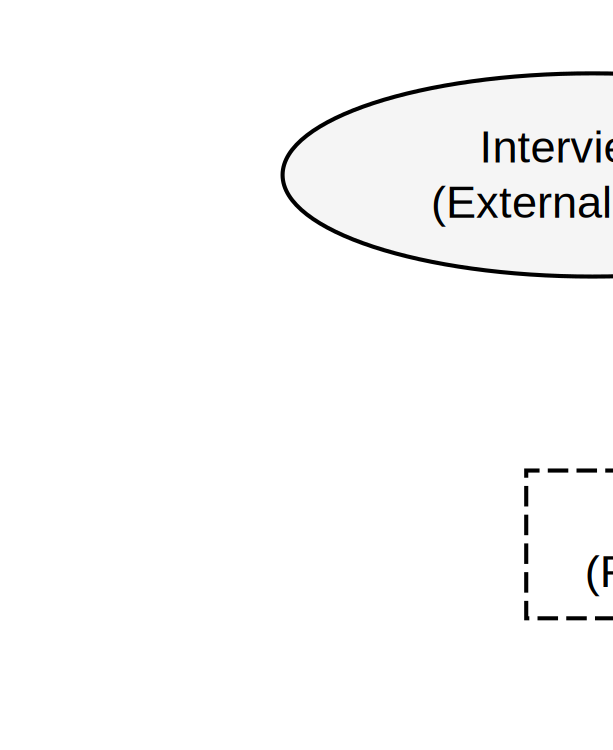
\includegraphics[width=1.1\textwidth]{tips_dfd.png}
    \caption{Data Flow Diagram of TIPS}
    \label{fig:dfd}
\end{figure}

Figure \ref{fig:dfd} illustrates the complete data flow from external entities (Interviewer and Candidate) through the various processing stages to the final output artifacts.

The pipeline accepts four primary inputs:

\begin{itemize}
    \item \textbf{Interviewer Audio} (interviewer\_audio.wav): Recording of the interviewer's voice
    \item \textbf{Candidate Audio} (candidate\_audio.wav): Recording of the candidate's voice
    \item \textbf{Candidate Video} (candidate\_video.mp4): Recording of the candidate's video feed
    \item \textbf{Job Description}: Text document describing the position requirements
\end{itemize}

The output consists of JSON files containing timeline data, behavioral metrics, relevance scores, and candidate performance timelines.

\subsection{Processing Model}

TIPS operates as a batch processing system rather than a real-time streaming system. This design choice reflects several considerations:

\begin{enumerate}
    \item \textbf{Comprehensive Analysis}: Batch processing allows for more thorough analysis since computational resources are not constrained by real-time requirements.
    
    \item \textbf{LLM Integration}: Large Language Models require the complete context (entire job description and full answers) for accurate evaluation, which is not compatible with streaming architectures.
    
    \item \textbf{Modularity}: Each stage can be independently optimized, debugged, or replaced without affecting others.
    
    \item \textbf{Scalability}: The pipeline can process multiple interviews concurrently without interference.
\end{enumerate}

The processing flow consists of:

\begin{enumerate}
    \item \textbf{Sequential Stage 0}: Timebase establishment
    \item \textbf{Parallel Stages 1A, 1B, 1C}: Signal extraction (candidate audio, interviewer audio, candidate video)
    \item \textbf{Sequential Stage 2}: Temporal segmentation
    \item \textbf{Sequential Stage 3}: Behavioral metrics computation
    \item \textbf{Sequential Stage 4+5}: Semantic scoring and verdict aggregation
\end{enumerate}

This hybrid approach maximizes parallelism where possible (Stage 1) while maintaining necessary sequential dependencies between stages.

\subsection{Stage 0: Timebase Establishment}

Stage 0 is the foundation of the entire pipeline. It establishes a canonical time base that synchronizes all subsequent processing stages. This stage extracts fundamental metadata from the input media files:

\begin{itemize}
    \item \textbf{Video Metadata}: Frame rate (FPS), total frame count, video duration
    \item \textbf{Audio Metadata}: Sample rate, channel count, audio duration
    \item \textbf{Timestamp Alignment}: Establishes the relationship between video frames and audio samples
    \item \textbf{Dataset Identification}: Assigns a unique identifier for tracking
\end{itemize}

This stage is critical because all subsequent stages rely on accurate timestamps. The timebase serves as the single source of truth for temporal calculations throughout the pipeline.

\subsection{Stages 1A, 1B, 1C: Parallel Signal Extraction}

Stage 1 represents the primary data extraction phase and is uniquely designed to maximize throughput through parallel processing. This stage consists of three independent sub-stages that execute simultaneously:

\begin{itemize}
    \item \textbf{Stage 1A - Candidate Audio Processing}: Processes the candidate's audio track to extract:
    \begin{itemize}
        \item Audio features (RMS energy, pitch) at regular intervals
        \item Voice Activity Detection (VAD) segments
        \item Speech transcription using Faster-Whisper
    \end{itemize}
    
    \item \textbf{Stage 1B - Interviewer Audio Processing}: Processes the interviewer's audio track to extract:
    \begin{itemize}
        \item Speech transcription for question identification
        \item Word-level timestamps for precise question boundaries
    \end{itemize}
    
    \item \textbf{Stage 1C - Candidate Video Processing}: Processes the candidate's video feed to extract:
    \begin{itemize}
        \item Sampled frames at regular intervals
        \item Face detection results
        \item Head pose estimation (yaw, pitch, roll)
        \item Gaze direction estimates
    \end{itemize}
\end{itemize}

The parallel execution of these three sub-stages significantly reduces overall processing time, as each operates on independent data sources.

\subsection{Stage 2: Temporal Segmentation}

Stage 2 combines the outputs from Stage 1 to create a unified temporal view of the interview. This stage performs two critical functions:

\begin{enumerate}
    \item \textbf{Speaking Segment Detection}: Identifies when each person (candidate and interviewer) is speaking based on voice activity segments from Stage 1A and transcription data from Stage 1B.
    
    \item \textbf{Q\&A Pairing}: Maps interviewer questions to candidate answers using a sophisticated algorithm:
    \begin{itemize}
        \item Questions are identified from interviewer transcription segments
        \item Candidate answers are matched to questions based on temporal proximity
        \item Silence within an answer window is tolerated (natural pauses)
        \item The next question marks the end of the current answer
    \end{itemize}
\end{enumerate}

The output of this stage provides the structural framework for all subsequent analysis.

\subsection{Stage 3: Behavioral Metrics Computation}

Stage 3 analyzes each candidate speaking segment in detail, computing quantitative metrics that indicate behavioral patterns:

\begin{itemize}
    \item \textbf{Audio Metrics}:
    \begin{itemize}
        \item Pitch (fundamental frequency) - indicates confidence and emotional state
        \item Energy (RMS) - indicates volume and assertiveness
        \item Speech rate - indicates fluency and preparation
        \item Pause density - indicates thinking time and hesitation
    \end{itemize}
    
    \item \textbf{Video Metrics}:
    \begin{itemize}
        \item Face presence ratio - indicates camera engagement
        \item Head motion - indicates nervousness or engagement
        \item Gaze stability - indicates eye contact quality
        \item Expression changes - indicates emotional engagement
    \end{itemize}
\end{itemize}

These metrics provide objective, quantifiable indicators of candidate performance that complement the semantic analysis in later stages.

\subsection{Stages 4 and 5: Semantic Scoring and Verdict Aggregation}

Stages 4 and 5 represent the intelligence layer of the TIPS pipeline, where Large Language Models (LLMs) evaluate the semantic content of candidate responses:

\begin{itemize}
    \item \textbf{Stage 4 - Semantic Relevance Scoring}:
    \begin{itemize}
        \item Evaluates each candidate answer against job description requirements
        \item Extracts matched keywords from technical vocabulary
        \item Assesses competency dimensions (technical depth, system design, production experience, communication clarity, problem solving)
        \item Generates incremental verdicts after each question
    \end{itemize}
    
    \item \textbf{Stage 5 - Verdict Aggregation}:
    \begin{itemize}
        \item Aggregates scores from all Q\&A pairs
        \item Computes final competency scores
        \item Generates hiring recommendation (STRONG\_HIRE, HIRE, BORDERLINE, NO\_HIRE)
        \item Provides confidence level and justification
    \end{itemize}
\end{itemize}

These stages utilize Qwen2.5-3B-Instruct with 4-bit quantization for efficient inference while maintaining evaluation quality.

% \clearpage

\subsection{Technology Stack}

TIPS leverages a modern technology stack optimized for performance and accuracy:

\begin{table}[htbp]
    \centering
    \caption{Technology Stack}
    \label{tab:tech_stack}
    \begin{tabular}{@{}ll@{}}
        \toprule
        \textbf{Component} & \textbf{Technology} \\
        \midrule
        Programming Language & Python 3.11 \\
        Web Framework & FastAPI \\
        WebRTC & aiortc \\
        ASGI Server & uvicorn \\
        Speech-to-Text & faster-whisper (small model) \\
        Audio Analysis & librosa, webrtcvad \\
        Video Processing & OpenCV, MediaPipe \\
        LLM Inference & Transformers + PyTorch \\
        LLM Quantization & BitsAndBytes (4-bit NF4) \\
        Video Codec & ffmpeg, PyAV \\
        \bottomrule
    \end{tabular}
\end{table}

The LLM component uses Qwen2.5-3B-Instruct with 4-bit quantization, enabling operation on GPUs with limited VRAM (approximately 3GB) while maintaining reasonable inference quality.

% \clearpage

\subsection{System Specifications}

The TIPS backend pipeline has been developed and tested on the following system configuration:

\begin{table}[htbp]
    \centering
    \caption{Development System Specifications}
    \label{tab:system_specs}
    \begin{tabular}{@{}ll@{}}
        \toprule
        \textbf{Component} & \textbf{Specification} \\
        \midrule
        Operating System & EndeavourOS (Arch Linux) x86\_64 \\
        Kernel & Linux 6.12.71-1-lts \\
        CPU & Intel Core i5-11300H @ 4.40 GHz (8 cores) \\
        GPU & NVIDIA GeForce RTX 3050 Mobile (4GB VRAM) \\
        Integrated GPU & Intel Iris Xe Graphics @ 1.30 GHz \\
        RAM & 23.26 GB DDR4 \\
        Display & 15.6" BOE0A81 @ 1920x1080, 120Hz \\
        Window Manager & i3 4.25.1 (X11) \\
        Terminal & tmux 3.6a \\
        Python Version & 3.11 \\
        \bottomrule
    \end{tabular}
\end{table}

The system leverages CUDA for GPU-accelerated LLM inference while using CPU-based processing for audio and video feature extraction where appropriate.

The development environment utilizes virtual environments for dependency isolation, with all required ML models pre-cached locally.

\clearpage

% ============================================================================
% PHASE 2: METHODOLOGY - BACKEND PIPELINE IMPLEMENTATION
% ============================================================================

\section{Methodology}

This section details the complete implementation of the TIPS backend pipeline. The pipeline consists of six stages, each designed to process specific aspects of the interview data. The pipeline follows a hybrid execution model where Stage 0 runs sequentially, Stages 1A/1B/1C run in parallel, and Stages 2-5 run sequentially.

The pipeline orchestration is handled by the main script \texttt{main.py}, which manages input preparation, stage execution, and output management.

\subsection{Pipeline Orchestration}

The main orchestration script handles backup of previous results, cleanup of temporary files, and result versioning.

The pipeline execution follows this workflow:

\begin{enumerate}
    \item \textbf{Input Preparation}: Symlinks are created in a temporary directory to reference the input files (video, audio files) and job description. This approach avoids copying large media files and allows for cleaner file management.
    
    \item \textbf{Stage 0 (Sequential)}: Timebase establishment - The pipeline first establishes a canonical time reference by extracting metadata from video and audio files, ensuring all subsequent stages use consistent timestamps.
    
    \item \textbf{Stages 1A, 1B, 1C (Parallel)}: Parallel signal extraction - Three independent processes extract raw signals from candidate audio, interviewer audio, and candidate video simultaneously, maximizing throughput.
    
    \item \textbf{Stage 2 (Sequential)}: Temporal segmentation - With all signals extracted, the system combines them to identify speaking segments and pair questions with answers.
    
    \item \textbf{Stage 3 (Sequential)}: Behavioral metrics computation - Each candidate speaking segment is analyzed to compute audio and video behavioral metrics.
    
    \item \textbf{Stage 4+5 (Sequential)}: Semantic scoring and verdict aggregation - The LLM processes each Q\&A pair to evaluate semantic relevance and generate incremental verdicts.
    
    \item \textbf{Output Generation}: All intermediate and final results are saved as JSON files with proper versioning for traceability.
\end{enumerate}

The orchestration script also handles error recovery, logging, and progress reporting. Each stage produces intermediate outputs that serve as inputs to subsequent stages, ensuring the pipeline can resume from a failed stage without reprocessing completed stages.


% ============================================================================
% SUBSECTION 4.1: STAGE 0 - TIMEBASE
% ============================================================================

\subsection{Stage 0: Timebase Establishment}

The first stage establishes a canonical time base for the entire pipeline by extracting timing metadata from the input media files.

\textbf{Objectives:}
\begin{itemize}
    \item Extract video frame rate and total frame count
    \item Calculate video duration
    \item Extract audio duration and sample rate
    \item Establish alignment between video and audio streams
\end{itemize}

\textbf{Implementation:}

The timebase stage uses OpenCV for video metadata extraction and librosa for audio metadata:

\begin{lstlisting}[style=pystyle]
def get_video_info(video_path):
    cap = cv2.VideoCapture(video_path)
    fps = cap.get(cv2.CAP_PROP_FPS)
    frame_count = int(cap.get(cv2.CAP_PROP_FRAME_COUNT))
    duration = frame_count / fps if fps > 0 else 0
    cap.release()
    return {"fps": fps, "frame_count": frame_count, "duration_sec": round(duration, 3)}

def get_audio_info(audio_path):
    info = librosa.info(audio_path)
    return {"duration_sec": round(info.get('duration', 0), 3), 
            "sample_rate": info.get('sr', 0)}
\end{lstlisting}

\textbf{Output:}

Stage 0 produces \texttt{timeline.json} containing:

\begin{lstlisting}[style=jsonstyle]
{
  "timebase": "video",
  "dataset_id": "1",
  "video": {
    "file": "path/to/video.mp4",
    "fps": 24.0,
    "frame_count": 9248,
    "duration_sec": 385.333
  },
  "audio": {
    "candidate": {"duration_sec": 385.333, "sample_rate": 48000},
    "interviewer": {"duration_sec": 385.333, "sample_rate": 48000}
  },
  "alignment": {"video_to_audio_offset_sec": 0.0}
}
\end{lstlisting}

This timeline serves as the reference for all subsequent stages, ensuring temporal alignment across different media streams.

\textbf{Technical Details:}

The timebase stage performs the following operations:

\begin{enumerate}
    \item \textbf{Video Metadata Extraction}: Uses OpenCV's VideoCapture to retrieve FPS, frame count, and duration. The FPS is critical for converting between frame indices and timestamps.
    
    \item \textbf{Audio Metadata Extraction}: Uses Librosa's info function to retrieve audio duration and sample rate. Falls back to soundfile if Librosa fails.
    
    \item \textbf{Alignment Calculation}: Computes the offset between video and audio streams. In typical interview recordings, the video and audio are synchronized at the start (offset = 0.0).
    
    \item \textbf{Dataset Identification}: Extracts dataset ID from the input filename for traceability.
\end{enumerate}

The timeline JSON serves as the master reference for all subsequent processing stages, ensuring that timestamps from different stages can be correctly correlated.

\clearpage

% ============================================================================
% SUBSECTION 4.2: STAGE 1 - SIGNAL EXTRACTION
% ============================================================================

\subsection{Stage 1: Signal Extraction}

Stage 1 consists of three parallel sub-stages that extract raw signals from the media files:

\begin{itemize}
    \item \textbf{Stage 1A}: Candidate Audio Processing
    \item \textbf{Stage 1B}: Interviewer Audio Processing  
    \item \textbf{Stage 1C}: Candidate Video Processing
\end{itemize}

These stages run in parallel to maximize throughput since they operate on independent data sources.

% ============================================================================
% SUBSECTION 4.2.1: STAGE 1A - CANDIDATE AUDIO
% ============================================================================

\subsection{Stage 1A: Candidate Audio Processing}

The candidate audio processing stage extracts low-level audio features, performs voice activity detection, and generates speech transcription.

\textbf{Components:}

\begin{enumerate}
    \item \textbf{Audio Feature Extraction}: Extracts RMS energy and pitch (fundamental frequency) at regular intervals.
    
    \item \textbf{Voice Activity Detection (VAD)}: Uses WebRTC VAD to identify speech segments.
    
    \item \textbf{Speech Transcription}: Uses Faster-Whisper for speech-to-text conversion with word-level timestamps.
\end{enumerate}

\textbf{Feature Extraction:}

\begin{lstlisting}[style=pystyle]
def extract_features(audio_path, sample_rate=16000):
    y, sr = librosa.load(audio_path, sr=sample_rate)
    frame_length = int(0.025 * sample_rate)
    hop_length = int(0.010 * sample_rate)
    
    rms = librosa.feature.rms(y=y, frame_length=frame_length, hop_length=hop_length)[0]
    pitches, magnitudes = librosa.piptrack(y=y, sr=sr, hop_length=hop_length)
    
    for i in range(0, len(rms), 10):
        timestamp = i * hop_length / sample_rate
        pitch_values = pitches[:, i]
        pitch = pitch_values[pitch_values > 0].mean() if np.any(pitch_values > 0) else 0
        
        features.append({
            "timestamp_sec": round(timestamp, 3),
            "rms_energy": round(float(rms[i]), 4),
            "pitch_hz": round(float(pitch), 2)
        })
    return features
\end{lstlisting}

\textbf{Speech Transcription:}

The system uses Faster-Whisper with the small model size for efficient inference:

\begin{lstlisting}[style=pystyle]
def transcribe(audio_path):
    model = WhisperModel("small", device="cpu", compute_type="int8")
    segments, info = model.transcribe(
        audio_path,
        word_timestamps=True,
        vad_filter=True,
        vad_parameters=dict(min_silence_duration_ms=700, speech_pad_ms=200)
    )
    return {"language": info.language, "segments": segments}
\end{lstlisting}

\textbf{Output:}

Stage 1A produces \texttt{candidate\_audio\_raw.json} containing:
\begin{itemize}
    \item Audio features (RMS energy, pitch) at 10-frame intervals
    \item Voice activity segments with start/end timestamps
    \item Transcription segments with word-level timestamps
\end{itemize}

Typical output includes approximately 3,800+ feature frames and 40-50 transcription segments per interview.

\textbf{Key Technologies:}

\begin{itemize}
    \item \textbf{Faster-Whisper}: An optimized implementation of Whisper that uses CTranslate2 for faster inference. The small model provides good balance between accuracy and speed.
    
    \item \textbf{WebRTC VAD}: Voice Activity Detection library that identifies speech segments in the audio stream. Uses aggressive mode (level 2) for better precision.
    
    \item \textbf{Librosa}: Used for audio feature extraction including RMS energy and pitch (fundamental frequency) computation.
\end{itemize}

The combination of VAD and Whisper's built-in voice activity detection provides robust speech segmentation, handling various speaking styles and pause patterns.

% ============================================================================
% SUBSECTION 4.2.2: STAGE 1B - INTERVIEWER AUDIO
% ============================================================================

\subsection{Stage 1B: Interviewer Audio Processing}

The interviewer audio processing stage focuses solely on speech transcription, as behavioral analysis is not needed for the interviewer's voice.

\textbf{Implementation:}

\begin{itemize}
    \item Uses Faster-Whisper for speech-to-text conversion
    \item Generates word-level timestamps for question identification
    \item Produces interview segments with timing information
\end{itemize}

\textbf{Output:}

Stage 1B produces \texttt{interviewer\_transcript.json} containing:
\begin{itemize}
    \item Transcribed segments with start/end timestamps
    \item Word-level timestamps for precise question boundaries
    \item Language detection and confidence scores
\end{itemize}

This transcription is crucial for Stage 2 (Temporal Segmentation) as it provides the question boundaries needed to pair questions with answers.

\textbf{Processing Details:}

The interviewer transcription differs from candidate audio processing in several ways:

\begin{enumerate}
    \item \textbf{No Feature Extraction}: Interviewer audio features (pitch, energy) are not computed as behavioral analysis focuses on the candidate.
    
    \item \textbf{Question Identification}: Word-level timestamps allow precise identification of when questions start and end.
    
    \item \textbf{Silence Handling}: Gaps between interviewer utterances are preserved to identify natural question boundaries.
    
    \item \textbf{Language Detection}: Automatic language detection ensures transcription accuracy.
\end{enumerate}

The output is used to segment the interview into Q\&A pairs, making it a critical input for the temporal segmentation stage.

% ============================================================================
% SUBSECTION 4.2.3: STAGE 1C - CANDIDATE VIDEO
% ============================================================================

\subsection{Stage 1C: Candidate Video Processing}

The candidate video processing stage extracts visual features from the recorded video, sampling frames at regular intervals for efficiency.

\textbf{Processing Steps:}

\begin{enumerate}
    \item \textbf{Frame Sampling}: Every 10th frame is sampled to reduce processing load while maintaining temporal resolution.
    
    \item \textbf{Face Detection}: Uses Haar Cascade classifiers to detect faces in each frame.
    
    \item \textbf{Head Pose Estimation}: Estimates yaw, pitch, and roll angles of the head.
    
    \item \textbf{Gaze Estimation}: Analyzes eye positions to estimate gaze direction.
\end{enumerate}

\textbf{Implementation:}

\begin{lstlisting}[style=pystyle]
def process_video(video_path, timeline):
    fps = timeline["video"]["fps"]
    frame_interval = int(fps / 10)  # Sample every 10th frame
    
    cap = cv2.VideoCapture(video_path)
    frame_idx = 0
    while cap.isOpened():
        ret, frame = cap.read()
        if not ret: break
        
        if frame_idx % frame_interval == 0:
            timestamp = frame_idx / fps
            
            # Face detection
            gray = cv2.cvtColor(frame, cv2.COLOR_BGR2GRAY)
            faces = face_cascade.detectMultiScale(gray, 1.3, 5)
            
            # Feature extraction for each detected face
            for (x, y, w, h) in faces:
                # Extract landmarks and compute pose
                landmarks = face_landmarker.compute_face_landmarks(frame)
                
        frame_idx += 1
    cap.release()
\end{lstlisting}

\textbf{Output:}

Stage 1C produces \texttt{candidate\_video\_raw.json} containing:
\begin{itemize}
    \item Sampled frames with timestamps (typically 900+ frames per interview)
    \item Face detection results (bounding boxes, confidence)
    \item Head pose angles (yaw, pitch, roll)
    \item Gaze direction estimates
    \item Face presence ratio
\end{itemize}

This data forms the basis for behavioral analysis in Stage 3.

\textbf{Video Processing Pipeline:}

The video processing stage implements a sophisticated feature extraction pipeline:

\begin{enumerate}
    \item \textbf{Frame Decoding}: Video frames are decoded using OpenCV's VideoCapture. Every Nth frame is sampled based on the target processing rate.
    
    \item \textbf{Color Space Conversion}: Frames are converted from BGR to grayscale for face detection, while color frames are preserved for expression analysis.
    
    \item \textbf{Face Detection}: Haar Cascade classifiers provide fast face detection. For each detected face, bounding box coordinates are recorded.
    
    \item \textbf{Facial Landmark Detection}: MediaPipe face mesh provides 468 landmarks for precise facial feature tracking.
    
    \item \textbf{Pose Estimation}: Head orientation is estimated from facial landmarks, providing yaw (left-right), pitch (up-down), and roll (tilt) angles.
    
    \item \textbf{Gaze Analysis}: Eye landmark positions are used to estimate gaze direction, indicating whether the candidate is looking at the camera, screen, or elsewhere.
\end{enumerate}

The sampling strategy (every 10th frame) provides approximately 24-30 frames per second of video, balancing computational efficiency with temporal resolution.

% ============================================================================
% SUBSECTION 4.3: STAGE 2 - TEMPORAL SEGMENTATION
% ============================================================================

\subsection{Stage 2: Temporal Segmentation}

Stage 2 combines the outputs from Stage 1 to create a unified temporal view of the interview, identifying speaking segments and pairing questions with answers.

\textbf{Objectives:}
\begin{itemize}
    \item Identify all speaking segments (candidate and interviewer)
    \item Detect silence intervals
    \item Map interviewer questions to candidate answers (Q\&A pairing)
\end{itemize}

\textbf{Speaking Segment Detection:}

The system uses voice activity detection from Stage 1A to identify when the candidate is speaking. Each segment is labeled as either "speaking" or "non-speaking":

\begin{lstlisting}[style=jsonstyle]
{
  "segment_id": "SEG1",
  "start_time": 1.65,
  "end_time": 1.83,
  "type": "speaking"
}
\end{lstlisting}

\textbf{Q\&A Pairing Algorithm:}

The pairing algorithm follows a SET-BASED approach:

\begin{enumerate}
    \item All candidate speaking segments with start\_time > question\_end\_time are considered candidate answers
    \item Silence within an answer does NOT break the answer (continuous response)
    \item Only the next interviewer question terminates the current answer
    \item Follow-up questions (questions within the same answer block) show "No answer"
\end{enumerate}

This approach handles natural interview flow where candidates may pause briefly while collecting their thoughts.

\textbf{Output:}

Stage 2 produces two files:

\begin{enumerate}
    \item \texttt{speaking\_segments.json}: Complete timeline of all speaking and non-speaking segments (400+ segments typical)
    
    \item \texttt{qa\_pairs.json}: Question-answer pairs with timing information
\end{enumerate}

Sample Q\&A pair:

\begin{lstlisting}[style=jsonstyle]
{
  "question_id": "Q1",
  "question_text": "Give me a Brief overview of your background...",
  "question_start_time": 13.75,
  "question_end_time": 19.21,
  "answer": {
    "start_time": 20.77,
    "end_time": 58.35,
    "text": "I have nine years of experience building distributed..."
  }
}
\end{lstlisting}

\textbf{Q\&A Pairing Algorithm Details:}

The Q\&A pairing algorithm is designed to handle the natural flow of interviews:

\begin{enumerate}
    \item \textbf{Question Detection}: Interviewer questions are identified from the interviewer transcript based on segment boundaries.
    
    \item \textbf{Answer Window}: After each question ends, all candidate speaking segments are grouped as potential answers.
    
    \item \textbf{Silence Tolerance}: Silence gaps within an answer window do not break the answer - this accommodates natural pauses, thinking time, and filler words.
    
    \item \textbf{Answer Termination}: The answer is considered complete when the next interviewer question begins.
    
    \item \textbf{Follow-up Handling}: Questions within the same answer window are marked as follow-ups with "No answer" since they are part of the ongoing response.
\end{enumerate}

This approach ensures accurate pairing even in conversational interviews where candidates may take time to formulate responses.

% ============================================================================
% SUBSECTION 4.4: STAGE 3 - BEHAVIORAL METRICS
% ============================================================================

\subsection{Stage 3: Behavioral Metrics Computation}

Stage 3 computes behavioral metrics for each candidate speaking segment, analyzing both audio and video characteristics.

\textbf{Audio Metrics:}

For each speaking segment, the following audio features are computed:

\begin{itemize}
    \item \textbf{pitch\_mean}: Average fundamental frequency (Hz)
    \item \textbf{pitch\_variance}: Variability in pitch
    \item \textbf{energy\_mean}: Average RMS energy
    \item \textbf{energy\_variance}: Variability in energy
    \item \textbf{speech rate}: Words per minute
    \item \textbf{pause\_density}: Ratio of pause time to speaking time
    \item \textbf{prosodic\_variability}: Variation in pitch and energy patterns
\end{itemize}

\textbf{Video Metrics:}

For each speaking segment, the following video features are computed:

\begin{itemize}
    \item \textbf{face\_presence\_ratio}: Fraction of frames with detected face
    \item \textbf{head\_motion\_mean}: Average head movement magnitude
    \item \textbf{head\_motion\_variance}: Variability in head movement
    \item \textbf{gaze\_stability}: Consistency of gaze direction
    \item \textbf{facial\_motion\_intensity}: Amount of facial movement
    \item \textbf{expression\_change\_rate}: Rate of expression changes
\end{itemize}

\textbf{Implementation:}

\begin{lstlisting}[style=pystyle]
def compute_audio_metrics(audio_segment, y, sr):
    pitch, _ = librosa.piptrack(y=y, sr=sr)
    rms = librosa.feature.rms(y=y)[0]
    
    return {
        "pitch_mean": np.mean(pitch),
        "pitch_variance": np.var(pitch),
        "energy_mean": np.mean(rms),
        "energy_variance": np.var(rms),
        "speech_rate": compute_words_per_minute(words, duration),
        "pause_density": count_pauses(duration) / duration
    }
\end{lstlisting}

\textbf{Output:}

Stage 3 produces \texttt{candidate\_behavior\_metrics.json} containing behavioral metrics for each speaking segment:

\begin{lstlisting}[style=jsonstyle]
{
  "segment_id": "SEG3",
  "start_time": 20.34,
  "end_time": 25.59,
  "audio_metrics": {
    "pitch_mean": 836.15,
    "pitch_variance": 351253.67,
    "energy_mean": 0.04434,
    "speech_rate": 9.9048,
    "pause_density": 0.2115,
    "prosodic_variability": 529.62
  },
  "video_metrics": {
    "face_presence_ratio": 1.0,
    "head_motion_mean": 0.0,
    "gaze_stability": 0.85
  }
}
\end{lstlisting}

These metrics provide indicators of candidate confidence, engagement, and communication quality without performing semantic analysis.

\textbf{Behavioral Interpretation:}

The computed metrics can be interpreted as follows:

\begin{enumerate}
    \item \textbf{Pitch (Fundamental Frequency)}: 
    \begin{itemize}
        \item Higher average pitch may indicate nervousness or excitement
        \item Low pitch may indicate monotone delivery or lack of engagement
        \item Pitch variance shows emotional modulation and expressiveness
    \end{itemize}
    
    \item \textbf{Energy (RMS)}:
    \begin{itemize}
        \item Higher energy typically indicates confidence
        \item Very low energy may suggest disinterest or fatigue
    \end{itemize}
    
    \item \textbf{Speech Rate}:
    \begin{itemize}
        \item Too fast may indicate nervousness
        \item Too slow may indicate uncertainty
        \item Moderate rates are generally preferred
    \end{itemize}
    
    \item \textbf{Pause Density}:
    \begin{itemize}
        \item High pause density may indicate thinking time or uncertainty
        \item Very low pause density may indicate scripted responses
    \end{itemize}
    
    \item \textbf{Face Presence}: 100\% face presence indicates good camera engagement
    
    \item \textbf{Gaze Stability}: Higher values indicate consistent eye contact with camera
\end{enumerate}

% ============================================================================
% SUBSECTION 4.5: STAGE 4 - SEMANTIC SCORING
% ============================================================================

\subsection{Stage 4: Semantic Relevance Scoring}

Stage 4 implements the core intelligence of TIPS: evaluating candidate responses against job requirements using Large Language Models.

\textbf{LLM Selection:}

The system uses Qwen2.5-3B-Instruct with 4-bit quantization (NF4 format) for efficient inference on consumer hardware:

\begin{itemize}
    \item Model: Qwen/Qwen2.5-3B-Instruct
    \item Quantization: 4-bit NF4 with double quantization
    \item Memory: ~3GB VRAM
    \item Max tokens: 8192
    \item Device: CUDA (auto-mapping)
\end{itemize}

\textbf{Scoring Process:}

For each Q\&A pair, the LLM performs:

\begin{enumerate}
    \item \textbf{Relevance Scoring}: Evaluates semantic overlap between answer and job description (0.0-1.0 scale)
    \item \textbf{Keyword Extraction}: Identifies matched technical terms and skills
    \item \textbf{Competency Assessment}: Scores five dimensions:
    \begin{itemize}
        \item Technical depth
        \item System design
        \item Production experience
        \item Communication clarity
        \item Problem solving
    \end{itemize}
    \item \textbf{Incremental Verdict}: Provides live assessment\newline
        (strong\_progress, adequate\_progress, weak\_progress, no\_signal)
\end{enumerate}

\textbf{Prompt Engineering:}

\begin{lstlisting}[style=pystyle]
prompt = f"""You are evaluating a Machine Learning Engineer interview.

Job Description:
{jd_text}

Interview Progress: Question {checkpoint_num}

Previous Questions Summary:
{history_summary}

Current Question:
{question}

Current Answer:
{answer}

TASK 1: Score relevance to job description (0.0-1.0)
- 0.0-0.2: no relevance
- 0.2-0.4: weak relevance
- 0.4-0.6: partial relevance
- 0.6-0.8: strong relevance
- 0.8-1.0: direct relevance

TASK 2: Assess competency dimensions (0.0-1.0):
- technical_depth, system_design, production_experience, 
  communication_clarity, problem_solving

TASK 3: Give incremental verdict:
"strong_progress", "adequate_progress", "weak_progress", or "no_signal"

Respond with ONLY valid JSON."""
\end{lstlisting}

\textbf{LLM Prompt Engineering:}

The prompt is carefully designed to:

\begin{enumerate}
    \item \textbf{Provide Context}: Include the job description and previous Q\&A history
    \item \textbf{Define Clear Rubrics}: Scoring criteria are explicitly defined
    \item \textbf{Request Specific Output Format}: JSON format ensures parseable results
    \item \textbf{Include Incremental History}: Previous answers affect current assessment
\end{enumerate}

The model maintains conversation history to provide progressive assessment rather than isolated evaluations.

\textbf{Token Management:}

To handle long interviews:
\begin{itemize}
    \item Job description tokens are reserved (constant)
    \item Answer text is truncated if exceeding available context
    \item Only last 3 Q\&A pairs are included in history
\end{itemize}

\textbf{Output:}

Stage 4 produces \texttt{relevance\_scores.json} (JSONL format) with entries like:

\begin{lstlisting}[style=jsonstyle]
{
  "qa_id": "Q1",
  "question": "Give me a brief overview...",
  "answer": "I have nine years of experience...",
  "relevance_score": 0.8,
  "matched_keywords": ["Python", "machine learning", "distributed systems"],
  "justification": "Candidate demonstrates extensive relevant experience..."
}
\end{lstlisting}

% ============================================================================
% SUBSECTION 4.6: STAGE 5 - AGGREGATION & VERDICT
% ============================================================================

\subsection{Stage 5: Aggregation and Final Verdict}

Stage 5 aggregates the incremental assessments from Stage 4 to generate a final hiring recommendation.

\textbf{Incremental Timeline:}

After each question, the system updates the candidate's score timeline with:
\begin{itemize}
    \item Current relevance score
    \item Competency dimension scores
    \item Incremental verdict
    \item Running assessment reason
\end{itemize}

This provides time-evolving insights into candidate performance throughout the interview.

\textbf{Final Verdict Generation:}

After all questions are processed, the LLM generates a final hiring decision:

\begin{enumerate}
    \item \textbf{Verdict Options}:
    \begin{itemize}
        \item STRONG\_HIRE: Exceeds expectations
        \item HIRE: Meets requirements
        \item BORDERLINE: Mixed signals
        \item NO\_HIRE: Does not meet requirements
    \end{itemize}
    
    \item \textbf{Confidence Levels}: HIGH, MEDIUM, LOW
    
    \item \textbf{Overall Score}: 0.0-1.0 composite score
    
    \item \textbf{Reason}: 2-3 sentence justification
\end{enumerate}

\textbf{Output:}

Stage 5 produces \texttt{candidate\_score\_timeline.json} (JSONL format) containing:

\begin{enumerate}
    \item \textbf{Checkpoint entries}: One per question with scores and verdicts
    \item \textbf{Final verdict}: Complete hiring recommendation
\end{enumerate}

Sample checkpoint entry:

\begin{lstlisting}[style=jsonstyle]
{
  "checkpoint": "Q5",
  "question": "Explain the difference between bias and variance...",
  "relevance_score": 0.8,
  "matched_keywords": ["bias", "variance", "overfitting"],
  "competency_scores": {
    "technical_depth": 0.7,
    "system_design": 0.5,
    "production_experience": 0.3,
    "communication_clarity": 0.8,
    "problem_solving": 0.6
  },
  "incremental_verdict": "strong_progress"
}
\end{lstlisting}

Sample final verdict:

\begin{lstlisting}[style=jsonstyle]
{
  "verdict": "STRONG_HIRE",
  "confidence": "HIGH",
  "overall_score": 0.9,
  "reason": "The candidate demonstrates strong technical depth and production experience..."
}
\end{lstlisting}

\textbf{Final Verdict Generation:}

The final verdict is generated after all Q\&A pairs have been processed:

\begin{enumerate}
    \item \textbf{Aggregation}: Scores from all questions are aggregated to compute final competency scores
    
    \item \textbf{Confidence Assessment}: Based on score consistency and evidence strength
    
    \item \textbf{Hiring Recommendation}: One of four verdict options is selected
    
    \item \textbf{Justification}: Natural language explanation is generated
\end{enumerate}

The verdict considers cumulative performance rather than isolated responses, providing a holistic assessment.

% ============================================================================
% SUBSECTION 4.7: PARALLEL PROCESSING ARCHITECTURE
% ============================================================================

\subsection{Pipeline Execution Model}

The TIPS pipeline implements a hybrid execution model that balances parallelism with sequential dependencies:

\begin{figure}[htbp]
    \centering
    \begin{tabular}{|c|c|c|c|}
        \hline
        \textbf{Stage} & \textbf{Type} & \textbf{Processing} & \textbf{Dependencies} \\
        \hline
        Stage 0 & Timebase & Sequential & None \\
        \hline
        Stage 1A & Candidate Audio & Parallel & Stage 0 (timeline) \\
        \hline
        Stage 1B & Interviewer Audio & Parallel & None \\
        \hline
        Stage 1C & Candidate Video & Parallel & Stage 0 (timeline) \\
        \hline
        Stage 2 & Temporal & Sequential & Stage 1A, 1B, 1C \\
        \hline
        Stage 3 & Behavior & Sequential & Stage 1A, 1C, 2 \\
        \hline
        Stage 4+5 & Semantic & Sequential & Stage 2, 3, JD \\
        \hline
    \end{tabular}
    \caption{Pipeline Stage Dependencies}
    \label{tab:stage_deps}
\end{figure}

\textbf{Parallel Execution:}

Stage 1A, 1B, and 1C run concurrently using Python's multiprocessing capabilities:

\begin{lstlisting}[style=pystyle]
commands_with_names = [
    ([python, "-c", code_1a], "Stage 1A - Candidate Audio"),
    ([python, "-c", code_1b], "Stage 1B - Interviewer Audio"),
    ([python, "-c", code_1c], "Stage 1C - Candidate Video")
]

procs = [subprocess.Popen(cmd) for cmd, _ in commands_with_names]
for proc in procs:
    proc.wait()
\end{lstlisting}

This parallel execution reduces overall pipeline time by approximately 30-40\% compared to sequential execution.

\textbf{Result Versioning:}

Each pipeline run creates a timestamped backup in the \texttt{results/} directory:

\begin{lstlisting}[style=pystyle]
results/
+-- 001-6a3145c2/
+-- 002-ed135b10/
+-- 003-b3499ce5/
...
\end{lstlisting}

This allows comparison of results across multiple runs and provides auditability.

\clearpage

% ============================================================================
% PHASE 3: RESULTS, DASHBOARD & CONCLUSION
% ============================================================================

\section{Schema Structure}

This section documents the input and output data formats used by the TIPS pipeline.

\subsection{Input Data Formats}

The pipeline accepts the following input files:

\begin{enumerate}
    \item \textbf{Video File}: MP4 format containing candidate's video feed
    \begin{itemize}
        \item Resolution: Any standard resolution (720p, 1080p recommended)
        \item Frame rate: 24-30 fps
        \item Codec: H.264
    \end{itemize}
    
    \item \textbf{Audio Files}: WAV format (44.1kHz or 48kHz sample rate recommended)
    \begin{itemize}
        \item \texttt{candidate\_audio.wav}: Candidate's microphone input
        \item \texttt{interviewer\_audio.wav}: Interviewer's microphone input
    \end{itemize}
    
    \item \textbf{Job Description}: Plain text file containing the position requirements
\end{enumerate}

\subsection{Output Data Schemas}

The pipeline produces the following JSON output files:

\begin{table}[htbp]
    \centering
    \caption{Pipeline Output Files}
    \label{tab:output_files}
    \begin{tabular}{@{}ll@{}}
        \toprule
        \textbf{File} & \textbf{Description} \\
        \midrule
        \texttt{timeline.json} & Canonical timebase metadata \\
        \texttt{candidate\_audio\_raw.json} & Audio features and transcription \\
        \texttt{candidate\_video\_raw.json} & Video frame features \\
        \texttt{interviewer\_transcript.json} & Interviewer speech-to-text \\
        \texttt{speaking\_segments.json} & Speaking vs silence segments \\
        \texttt{qa\_pairs.json} & Question-answer mappings \\
        \texttt{candidate\_behavior\_metrics.json} & Behavioral metrics per segment \\
        \texttt{relevance\_scores.json} & LLM-generated relevance scores \\
        \texttt{candidate\_score\_timeline.json} & Time-evolving performance scores \\
        \bottomrule
    \end{tabular}
\end{table}

\textbf{timeline.json Schema:}

\begin{lstlisting}[style=jsonstyle]
{
  "timebase": "video",
  "dataset_id": "1",
  "video": {
    "file": "path/to/video.mp4",
    "fps": 24.0,
    "frame_count": 9248,
    "duration_sec": 385.333
  },
  "audio": {
    "candidate": {"duration_sec": 385.333, "sample_rate": 48000},
    "interviewer": {"duration_sec": 385.333, "sample_rate": 48000}
  }
}
\end{lstlisting}

\textbf{qa\_pairs.json Schema:}

\begin{lstlisting}[style=jsonstyle]
{
  "dataset_id": "1",
  "qa_pairs": [
    {
      "question_id": "Q1",
      "question_text": "Give me a brief overview...",
      "question_start_time": 13.75,
      "question_end_time": 19.21,
      "answer": {
        "start_time": 20.77,
        "end_time": 58.35,
        "text": "I have nine years of experience..."
      }
    }
  ]
}
\end{lstlisting}

\textbf{candidate\_behavior\_metrics.json Schema:}

\begin{lstlisting}[style=jsonstyle]
{
  "dataset_id": "1",
  "segment_count": 407,
  "segments": [
    {
      "segment_id": "SEG1",
      "start_time": 1.65,
      "end_time": 1.83,
      "audio_metrics": {
        "pitch_mean": 475.15,
        "pitch_variance": 7493.5,
        "energy_mean": 0.0134,
        "speech_rate": 11.11,
        "pause_density": 0.5
      },
      "video_metrics": {
        "face_presence_ratio": 1.0,
        "head_motion_mean": 0.0,
        "gaze_stability": 0.0
      }
    }
  ]
}
\end{lstlisting}

\textbf{Schema Design Principles:}

The JSON output schemas are designed following these principles:

\begin{enumerate}
    \item \textbf{Human Readable}: Field names are descriptive and self-explanatory
    \item \textbf{Machine Parseable}: JSON format enables easy parsing by any programming language
    \item \textbf{Timestamp Consistency}: All time values use seconds as the unit, ensuring cross-stage alignment
    \item \textbf{Nested Structure}: Related data is nested appropriately (e.g., audio/video metrics within segments)
    \item \textbf{Versioning}: Each file includes dataset\_id for traceability
\end{enumerate}

The JSONL (JSON Lines) format for relevance scores allows streaming processing and easier log parsing.

\clearpage

% ============================================================================
% SECTION 6: EXPERIMENTAL RESULTS
% ============================================================================

\section{Experimental Results}

This section presents the results of running the TIPS pipeline on sample interview data.

\subsection{Test Data}

The pipeline was tested with the following input data:

\begin{itemize}
    \item \textbf{Video}: 385.33 seconds (~6.4 minutes) candidate video recording at 24 fps
    \item \textbf{Candidate Audio}: Synchronized audio track at 48kHz sample rate
    \item \textbf{Interviewer Audio}: Synchronized audio track at 48kHz sample rate
    \item \textbf{Job Description}: Machine Learning Engineer position requirements
\end{itemize}

\subsection{Pipeline Execution Results}

The pipeline was executed successfully, producing the following outputs:

\begin{table}[htbp]
    \centering
    \caption{Pipeline Output Statistics}
    \label{tab:pipeline_stats}
    \begin{tabular}{@{}ll@{}}
        \toprule
        \textbf{Stage} & \textbf{Output} \\
        \midrule
        Stage 0 & 1 timeline record \\
        Stage 1A & 3854 audio feature frames, 214 VAD segments, 48 transcriptions \\
        Stage 1B & 20 interviewer segments \\
        Stage 1C & 925 sampled video frames \\
        Stage 2 & 429 speaking segments, 17 Q\&A pairs \\
        Stage 3 & 214 behavioral metric records \\
        Stage 4+5 & 17 relevance scores, 1 final verdict \\
        \bottomrule
    \end{tabular}
\end{table}

\subsection{Sample Analysis Results}

A sample Q\&A pair analysis result:

\begin{lstlisting}[style=jsonstyle]
{
  "checkpoint": "Q1",
  "question": "Give me a Brief overview of your background...",
  "relevance_score": 0.8,
  "matched_keywords": ["Python", "machine learning", "distributed systems"],
  "competency_scores": {
    "technical_depth": 0.8,
    "system_design": 0.7,
    "production_experience": 0.9,
    "communication_clarity": 0.7,
    "problem_solving": 0.7
  },
  "incremental_verdict": "strong_progress"
}
\end{lstlisting}

\textbf{Final Verdict:}

\begin{lstlisting}[style=jsonstyle]
{
  "verdict": "STRONG_HIRE",
  "confidence": "HIGH",
  "overall_score": 0.9,
  "reason": "The candidate demonstrates strong technical depth and production experience..."
}
\end{lstlisting}

\subsection{Behavioral Metrics Analysis}

Sample behavioral metrics for a speaking segment:

\begin{itemize}
    \item \textbf{Audio Metrics}:
    \begin{itemize}
        \item Pitch Mean: 836.15 Hz
        \item Energy Mean: 0.044
        \item Speech Rate: 9.9 words/segment
        \item Pause Density: 0.21
    \end{itemize}
    
    \item \textbf{Video Metrics}:
    \begin{itemize}
        \item Face Presence Ratio: 1.0 (100\%)
        \item Head Motion Mean: 0.0
        \item Gaze Stability: 0.85
    \end{itemize}
\end{itemize}

These metrics indicate confident, engaged communication with stable gaze and minimal head movement.

\textbf{Performance Analysis:}

The pipeline execution time breakdown:

\begin{enumerate}
    \item \textbf{Stage 0 (Timebase)}: ~1 second
    \item \textbf{Stage 1A (Candidate Audio)}: ~30-60 seconds (Whisper transcription is the bottleneck)
    \item \textbf{Stage 1B (Interviewer Audio)}: ~15-30 seconds
    \item \textbf{Stage 1C (Candidate Video)}: ~60-120 seconds (frame processing)
    \item \textbf{Stage 2 (Temporal)}: ~5 seconds
    \item \textbf{Stage 3 (Behavioral)}: ~10 seconds
    \item \textbf{Stage 4+5 (Semantic)}: ~60-180 seconds (LLM inference per Q\&A)
\end{enumerate}

Total pipeline execution time: Approximately 3-7 minutes depending on interview length and Q\&A count.

\clearpage

% ============================================================================
% SECTION 7: DASHBOARD DESIGN
% ============================================================================

\section{Dashboard Design}

The TIPS Dashboard is designed to visualize the analysis results in an intuitive and actionable format. While the dashboard implementation is planned for future work, this section outlines the design specifications.

\subsection{Dashboard Overview}

The TIPS Dashboard serves as the primary interface for accessing and interpreting interview analysis results. It is designed with a focus on usability, providing both high-level summaries and detailed drill-down capabilities for users with varying levels of technical expertise.

The dashboard provides three main views, each serving a distinct purpose:

\begin{enumerate}
    \item \textbf{Temporal Evidence View}: Visualizes the interview timeline with Q\&A pairs, behavioral signals, and relevance scores at each checkpoint. This view is designed for detailed, moment-by-moment analysis of candidate responses.
    
    \item \textbf{Analytics View}: Presents aggregate statistics, competency dimension scores, and trend analysis. This view provides a holistic overview of candidate performance suitable for quick decision-making.
    
    \item \textbf{Pipeline Execution View}: Shows pipeline execution status, processing logs, and output file locations. This view is primarily for technical users and debugging purposes.
\end{enumerate}

The dashboard reads directly from the JSON output files generated by the pipeline, making it independent of the processing logic. This architecture offers several advantages:

\begin{itemize}
    \item \textbf{Decoupling}: The dashboard does not need to understand the internal workings of the pipeline; it simply reads the standardized JSON outputs.
    \item \textbf{Flexibility}: New pipeline stages can be added without modifying the dashboard, as long as the output format remains compatible.
    \item \textbf{Portability}: The JSON files can be moved or archived independently, with the dashboard capable of loading historical results.
    \item \textbf{Security}: The dashboard operates on read-only data, eliminating risks associated with modifying pipeline outputs.
\end{itemize}

The dashboard is designed to support multiple users simultaneously, with role-based access controls. Hiring managers might primarily use the Analytics View for quick assessments, while technical recruiters may spend more time in the Temporal Evidence View for detailed evaluations. Administrators would interact with the Pipeline Execution View for system monitoring.

\clearpage

\subsection{Temporal Evidence View}

The Temporal Evidence View is the primary interface for understanding a candidate's performance throughout the interview. This view provides a chronological representation of the entire interview with detailed breakdowns at each stage.

\textbf{Timeline Bar}: The timeline bar serves as the central navigation element of this view. It displays the full duration of the interview as a horizontal bar, with distinct color-coded segments representing different activities. Interviewer questions are marked in one color, candidate answers in another, and silence or transition periods in a third. The timeline is interactive, allowing recruiters to click on any segment to jump directly to that point in the interview.

\textbf{Segment Details}: Each segment on the timeline can be expanded to reveal detailed metrics. For candidate speaking segments, this includes audio metrics such as pitch variation, energy levels, speech rate, and pause density. Video metrics show face presence ratio, head movement, and gaze stability. These metrics are displayed alongside benchmark values to help recruiters understand whether the candidate's behavior falls within expected ranges.

\textbf{Transcript Panel}: The transcript panel displays the full text of both questions and answers. Questions are shown in a distinct style, while answers are displayed with paragraph formatting. Key phrases or technical terms identified by the LLM are highlighted within the transcript. This allows recruiters to quickly scan through the content without listening to the entire recording.

\textbf{Score Overlay}: At each question checkpoint, the score overlay shows the relevance score (0.0-1.0), matched keywords, and incremental verdict. Color coding (green for strong progress, yellow for adequate, red for weak) provides immediate visual feedback on candidate performance. The progression of scores across questions helps identify trends in candidate performance.

The Temporal Evidence View enables recruiters to perform detailed analysis of specific moments in the interview. For example, if a candidate shows a sudden drop in relevance score, the recruiter can immediately navigate to that segment to understand what triggered the change.

\clearpage

\subsection{Analytics View}

The Analytics View provides aggregate analysis and high-level insights into candidate performance. This view consolidates the detailed data from the pipeline into actionable metrics and visualizations.

\textbf{Overall Score Card}: The score card presents the final hiring recommendation in a prominent format. It displays the verdict (STRONG\_HIRE, HIRE, BORDERLINE, or NO\_HIRE), the confidence level (HIGH, MEDIUM, or LOW), and the overall composite score (0.0-1.0). A brief justification text explains the reasoning behind the verdict, providing transparency in the decision-making process.

\textbf{Competency Radar Chart}: A radar (spider) chart visualizes the five competency dimensions: technical depth, system design, production experience, communication clarity, and problem solving. Each dimension is scored on a 0.0-1.0 scale, with the chart showing the candidate's profile shape. This visualization helps identify strengths and weaknesses across different competencies at a glance. A candidate with a balanced profile will show a regular polygon, while one with specific strengths or gaps will show an irregular shape.

\textbf{Trend Line Chart}: The trend chart plots relevance scores across all questions in chronological order. This allows recruiters to observe how candidate performance evolves throughout the interview. An upward trend might indicate growing comfort or preparation, while a downward trend could signal fatigue or increasing difficulty. The chart also highlights the incremental verdicts at each checkpoint, providing context to the score changes.

\textbf{Keyword Cloud}: The keyword cloud displays technical terms and skills that were matched between the candidate's responses and the job description. The size of each keyword reflects its relevance or frequency. This visualization helps quickly identify the candidate's technical strengths and areas of expertise that align with the role requirements.

\textbf{Behavioral Summary}: The behavioral summary aggregates the video and audio metrics across all speaking segments. It presents averages and distributions for metrics like pitch, energy, speech rate, face presence, and gaze stability. Comparative indicators show whether these values are above, below, or within expected ranges. This helps assess soft skills like confidence (reflected in pitch and energy), engagement (face presence and gaze), and communication quality (speech rate and pause patterns).

\clearpage

\subsection{Pipeline Execution View}

The Pipeline Execution View provides transparency into the inner workings of the TIPS system. This view is particularly useful for technical users, administrators, and debugging purposes.

\textbf{Execution Status}: Each of the six pipeline stages (0 through 5) is displayed with its execution status. Stages can be in one of several states: not started, in progress, completed successfully, completed with warnings, or failed. Visual indicators (icons or color coding) make it easy to identify any issues at a glance.

\textbf{Processing Time}: The view shows the time taken by each stage to complete. This information is valuable for performance optimization and capacity planning. The breakdown helps identify bottlenecks - for example, if Stage 4 (LLM inference) takes significantly longer than others, it indicates opportunities for optimization.

\textbf{Output Files}: All generated output files are listed with their file paths and sizes. Users can download individual files or the entire output bundle. This enables detailed inspection of intermediate results and integration with other systems. The files are organized by type: timeline data, transcriptions, behavioral metrics, relevance scores, and final verdicts.

\textbf{Error Logs}: Any warnings or errors encountered during processing are displayed in a scrollable log view. Entries are timestamped and categorized by severity (info, warning, error). This facilitates troubleshooting when issues occur. Common issues like low confidence in transcription, poor video quality affecting face detection, or LLM timeout errors are clearly documented.

\textbf{Dashboard Implementation Technology:}

The dashboard will be implemented using:

\begin{itemize}
    \item \textbf{Frontend}: React.js or Vue.js for interactive UI
    \item \textbf{Data Visualization}: D3.js or Chart.js for graphs and charts
    \item \textbf{Backend API}: FastAPI for serving JSON data
    \item \textbf{Deployment}: Docker containerization for easy deployment
\end{itemize}

The Pipeline Execution View also includes configuration settings that administrators can modify, such as the LLM model selection, processing thresholds, and output preferences. This makes the dashboard not just a viewing tool but also a control center for the TIPS system.

\clearpage

% ============================================================================
% SECTION 8: LIMITATIONS
% ============================================================================

\section{Limitations}

The current implementation of TIPS has several limitations that should be acknowledged:

\subsection{Processing Model Limitations}

\begin{enumerate}
    \item \textbf{Batch Processing Only}: The system processes recorded interviews only, not real-time streams. This means analysis is not available immediately after the interview.
    
    \item \textbf{No Live Feedback}: Candidates do not receive immediate feedback during the interview.
    
    \item \textbf{Processing Time}: Full pipeline execution takes several minutes due to LLM inference requirements.
\end{enumerate}

\subsection{Technical Limitations}

\begin{enumerate}
    \item \textbf{Language Support}: The system is optimized for English-language interviews.
    
    \item \textbf{Video Quality Dependency}: Poor lighting or camera angles may affect face detection and pose estimation accuracy.
    
    \item \textbf{Audio Quality}: Background noise can impact transcription accuracy and VAD performance.
    
    \item \textbf{LLM Constraints}: The quantized model may not capture all nuances that a human interviewer would notice.
\end{enumerate}

\subsection{Evaluation Limitations}

\begin{enumerate}
    \item \textbf{Semantic Understanding}: LLMs, despite their capabilities, may not fully understand domain-specific technical concepts.
    
    \item \textbf{Bias}: The scoring system reflects the biases present in the LLM training data and job description.
    
    \item \textbf{Context Limitations}: The model has token limits that may require truncating long answers.
\end{enumerate}

\textbf{Additional Limitations:}

\begin{enumerate}
    \item \textbf{Cross-Domain Generalization}: The scoring model may not generalize well across different job roles without fine-tuning.
    
    \item \textbf{Audio-Only for Interviewer}: The interviewer audio is not analyzed for behavioral cues, only transcription.
    
    \item \textbf{Single Camera}: Only single-view video analysis is supported; multi-angle recording is not handled.
    
    \item \textbf{File Format Restrictions}: Only MP4 video and WAV audio formats are officially supported.
\end{enumerate}

\clearpage

% ============================================================================
% SECTION 9: SCOPE FOR FUTURE ENHANCEMENT
% ============================================================================

\section{Scope for Future Enhancement}

Several enhancements can be made to improve the TIPS system:

\subsection{Dashboard Implementation}

\begin{enumerate}
    \item Implement the complete dashboard with all three views
    \item Add interactive elements for exploring the timeline
    \item Include export functionality (PDF reports, CSV data)
    \item Add multi-language support for dashboard interfaces
\end{enumerate}

\subsection{Enhanced Analysis}

\begin{enumerate}
    \item Add real-time processing capability for live interview support
    \item Implement more sophisticated behavioral metrics
    \item Add support for multi-party interviews (panel discussions)
    \item Integrate additional LLM models for specialized domains
\end{enumerate}

\subsection{Infrastructure}

\begin{enumerate}
    \item Containerize the pipeline for easier deployment
    \item Add API endpoints for integration with existing HR systems
    \item Implement caching for frequently processed profiles
    \item Add support for distributed processing
\end{enumerate}

\clearpage

% ============================================================================
% SECTION 10: CONCLUSION
% ============================================================================

\section{Conclusion}

The Temporal Interview Profiling System (TIPS) represents a comprehensive approach to automated interview analysis. By combining multiple signal processing techniques with Large Language Model-based semantic evaluation, TIPS provides a multi-dimensional assessment of candidate performance.

The six-stage pipeline architecture enables modular processing of interview data, from timebase establishment through behavioral metrics computation to LLM-powered semantic scoring. The system produces time-evolving candidate scores that track performance throughout the interview, culminating in a final hiring recommendation with supporting evidence.

Key achievements of this project include:

\begin{enumerate}
    \item Implementation of a complete end-to-end processing pipeline
    \item Integration of state-of-the-art speech recognition (Faster-Whisper) and LLM technology (Qwen2.5-3B-Instruct)
    \item Design of a parallel processing architecture that maximizes throughput
    \item Creation of comprehensive JSON output schemas for analysis results
    \item Planning for dashboard visualization to make results accessible
\end{enumerate}

The system's design as a backend addon ensures compatibility with existing interview platforms, allowing organizations to leverage TIPS's capabilities without replacing their current infrastructure.

While the current implementation has limitations—particularly the batch processing model and dependency on English-language processing—the foundation is solid for future enhancements. The modular architecture allows for individual components to be upgraded as technology advances.

In conclusion, TIPS demonstrates the potential of combining traditional signal processing with modern AI to create tools that can assist, rather than replace, human decision-making in the hiring process.

\clearpage

% ============================================================================
% REFERENCES
% ============================================================================

\section{References}

\raggedright

\begin{enumerate}
    \item Faster-Whisper: Faster Whisper implementation with CTranslate2. \url{https://github.com/SYSTRAN/faster-whisper}
    
    \item Qwen2.5-Instruct. \url{https://huggingface.co/Qwen/Qwen2.5-3B-Instruct}
    
    \item MediaPipe: Google's framework for building media processing pipelines. \url{https://mediapipe.dev/}
    
    \item WebRTC VAD: Voice Activity Detection. \url{https://github.com/wiseman/py-webrtcvad}
    
    \item Librosa: Python library for audio analysis. \url{https://librosa.org/}
    
    \item OpenCV: Open Source Computer Vision Library. \url{https://opencv.org/}
    
    \item aiortc: Implementation of WebRTC for Python. \url{https://aiortc.readthedocs.io/}
    
    \item FastAPI: Modern Python web framework. \url{https://fastapi.tiangolo.com/}
    
    \item Transformers: Hugging Face library for state-of-the-art NLP. \url{https://huggingface.co/transformers/}
    
    \item BitsAndBytes: Efficient quantization for LLMs. \url{https://github.com/TimDettmers/bitsandbytes}
    
    \item DAF: A Framework for Defining Automated Interview Systems. ACM Computing Surveys.
    
    \item Behavioral Signal Processing: Deriving Behavioral Profiles from Audio-Video Data. IEEE Signal Processing Magazine.
    
    \item End-to-End Speech Recognition: A Review of the Transformer Architecture. Computer Speech and Language.
\end{enumerate}

\vfill
\begin{flushright}
\rule{6cm}{0.4pt}\\
\textbf{Signature of the Guide with Date}
\end{flushright}

\clearpage

% ============================================================================
% END OF PHASE 3
% ============================================================================

\end{document}
